\documentclass[12pt,a4paper]{report}
\usepackage{amsmath}
\usepackage{amsfonts}
\usepackage{amssymb}
\usepackage{fullpage}
\usepackage[slovak]{babel}
\usepackage[utf8]{inputenc}
\usepackage[T1]{fontenc}
\usepackage{fullpage}
\usepackage{indentfirst}
\usepackage{array}
\usepackage{caption}
\usepackage{graphicx}
\usepackage{placeins}
\DeclareGraphicsExtensions{.png,.jpg}

\begin{document}
\begin{titlepage}
\centering\bfseries
		Fakulta matematiky, fyziky a informatiky\\Univerzita Komenského v Bratislave	
	\vspace*{\stretch{2.0}}

	\fontsize{23}{28}\textbf{Špecifikácia požiadaviek na softvér}\\
	\vspace*{\stretch{0.05}}
	\fontsize{16}{22}\textbf{Predikcia šírenia infekčných ochorení}\\
	\vspace*{\stretch{0.2}}
	\large\textit{Matúš Čongrády\\Tibor Hanesz\\Jonatan Foltyn\\Katarína Šimnová}

	\vspace*{\stretch{2.0}}
\end{titlepage}\bigskip
	\setcounter{tocdepth}{9}
	\tableofcontents
	
\renewcommand{\chaptername}{}	
\chapter[Konceptuálna analýza]{\rmfamily\bfseries
	Konceptuálna analýza}
	
\section[Používateľské rozhranie]{\rmfamily\bfseries
	Používateľské rozhranie}
Táto  časť  bude  venovaná približnému  grafickému  opisu užívateľského  rozhrania. Opisuje aké komponenty sa budú nachádzať na akých stránkach a čo bude ich želaným vstupom.

\subsection[Hlavná stránka]{\rmfamily\bfseries
	Hlavná stránka}

\begin{figure}[htb]
	\centering
	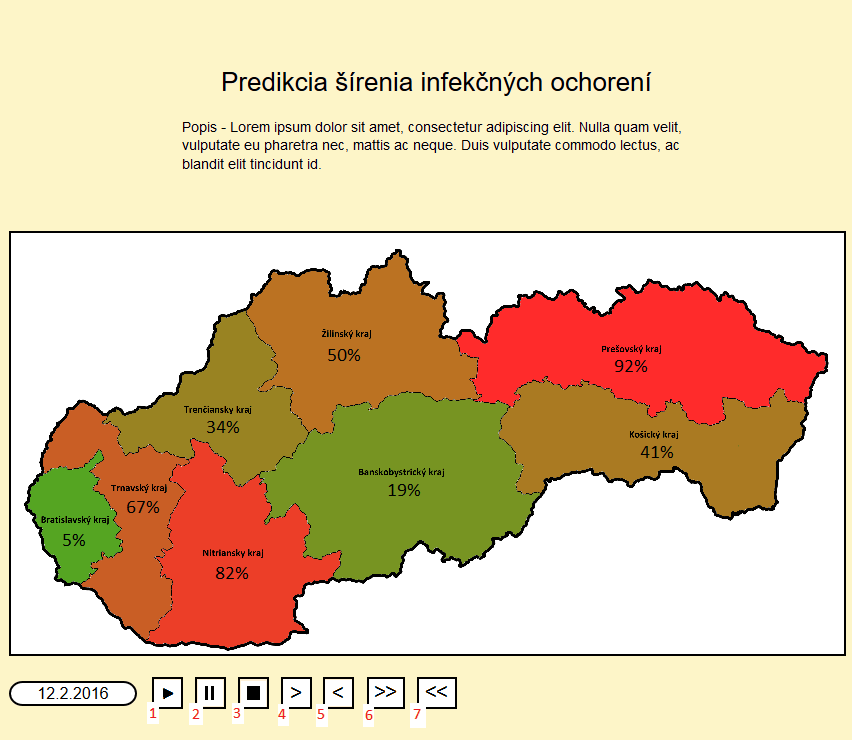
\includegraphics[scale=0.55]{hl_stranka}
	\caption{Hlavná stránka}
	\label{fig:Hlavná stránka}
\end{figure}


\begin{table}[h!]
	\centering
	\begin{tabular}{|>{\centering\arraybackslash}m{3in}|>{\centering\arraybackslash}m{3in}|}
		\hline
		\centering Parameter & Vlastnosti \\ [0ex]
		\hline
		Mapa & Miesto zobrazenia animácie šírenia infekčného ochorenia.\\ [0ex]
		\hline
		0. &  Označuje deň, pre ktorý animacácia v danom momente zobrazuje štatistiku.\\ [0ex]
		\hline
		1. & Spustenie animácie.\\ [0ex]	
		\hline
		2. & Zastavenie animácie.\\ [0ex]	
		\hline
		3. & Vypnutie animácie.\\ [0ex]	
		\hline
		4. & Prechod o jeden deň vpred.\\ [0ex]	
		\hline
		5. & Prechod o jeden deň vzad.\\ [0ex]	
		\hline
		6. & Zrýchlenie animácie.\\ [0ex]	
		\hline
		7. & Spomalenie animácie.\\ [0ex]	
		\hline

	\end{tabular}
\end{table}
\FloatBarrier
\pagebreak
\subsection[Prihlásenie]{\rmfamily\bfseries
	Prihlásenie}

\begin{figure}[htb]
	\centering
	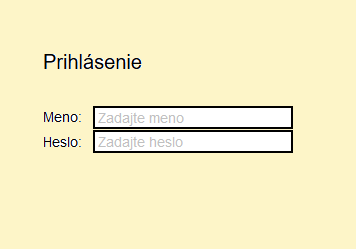
\includegraphics[scale=0.6]{prihlasenie}
	\caption{Prihlásenie}
	\label{fig:Prihlásenie}
\end{figure}


\begin{table}[h!]
	\centering
	\begin{tabular}{|>{\centering\arraybackslash}m{3in}|>{\centering\arraybackslash}m{3in}|}
		\hline
		\centering Parameter & Vlastnosti \\ [0ex]
		\hline
		Heslo & Užívateľ zadá svoje prihlasovacie heslo. \\ [0ex]
		\hline
	\end{tabular}
\end{table}
\FloatBarrier
\subsection[Administrácia]{\rmfamily\bfseries
	Administrácia}

\begin{figure}[!h]
	\centering
	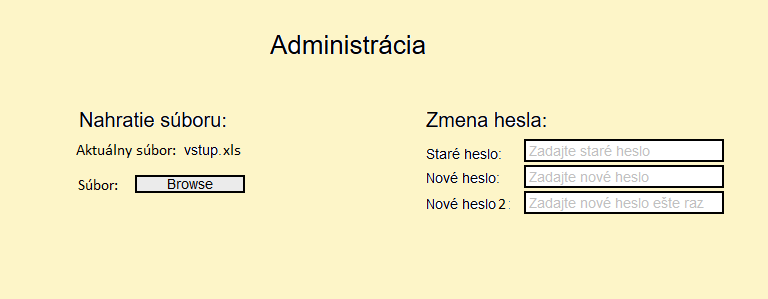
\includegraphics[scale=0.7]{admin}
	\caption{Administrácia}
	\label{fig:Administrácia}
\end{figure}

\begin{table}[h!]
	\centering
	\begin{tabular}{|>{\centering\arraybackslash}m{3in}|>{\centering\arraybackslash}m{3in}|}
		\hline
		\centering Parameter & Vlastnosti \\ [0ex]
		\hline
		Aktuálny súbor & Návestie zobrazujúce názov súboru aktuálne použitého vstupu.\\ [0ex]
		\hline
		Súbor & Užívateľ  vyberie  validný XLS súbor obsahujúci maticu. \\ [0ex]
		\hline
		Staré heslo & Užívateľ zadá svoje pôvodné heslo.\\ [0ex]	
		\hline
		Nové heslo & Užívateľ zadá svoje nové heslo. \\ [0ex]		
		\hline
		Nové heslo 2 & Užívateľ zadá svoje nové heslo druhýkrát. \\ [0ex]		
		\hline
	\end{tabular}
\end{table}
\FloatBarrier
\pagebreak
\section[Možnosti užívateľa]{\rmfamily\bfseries
	Možnosti užívateľa}

	V tejto časti sú umiestnené diagramy, ktoré popisujú predovšetkým možné činnosti užívateľa resp. administrátora v systéme.

\subsection[Stavový diagram]{\rmfamily\bfseries
	Stavový diagram}
Tento diagram ukazuje jednotlivé stavy a ich zmeny v troch situáciách:
\begin{itemize}
	\item prezeranie prezentácie
	\item zmena hesla,
	\item zmena údajov, z ktorých sa vytvára animácia.
\end{itemize}
\begin{figure}[htb]
	\centering
	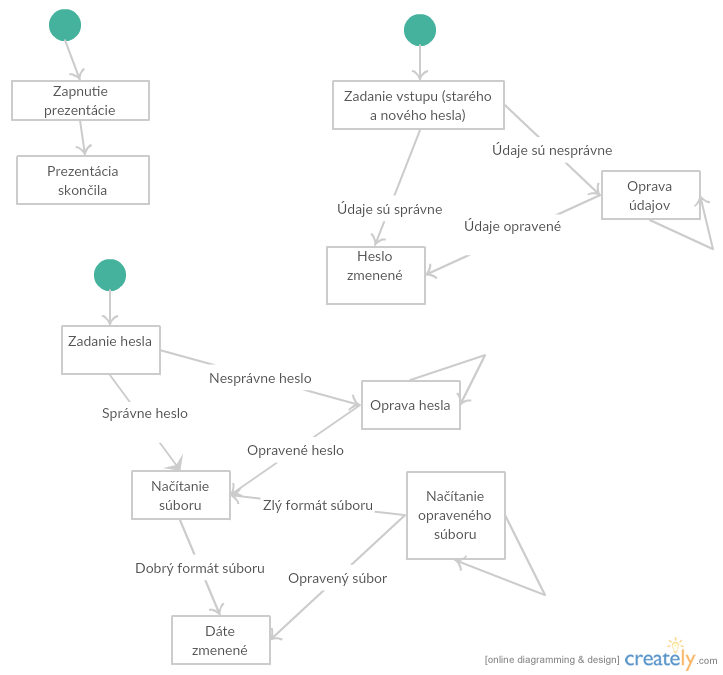
\includegraphics[scale=0.5]{Stavovy_diagram}
	\caption{Stavový diagram}
	\label{fig:Stavový diagram}
\end{figure}
\FloatBarrier
\clearpage
\subsection[Use case diagram]{\rmfamily\bfseries
	Use case diagram}
	Tento diagram poskytuje najzákladnejší prehľad prípadov použitia. Každý prípad použitia opisuje jeden spôsob použitia systému z hľadiska používateľa

\begin{figure}[htb]
	\centering
	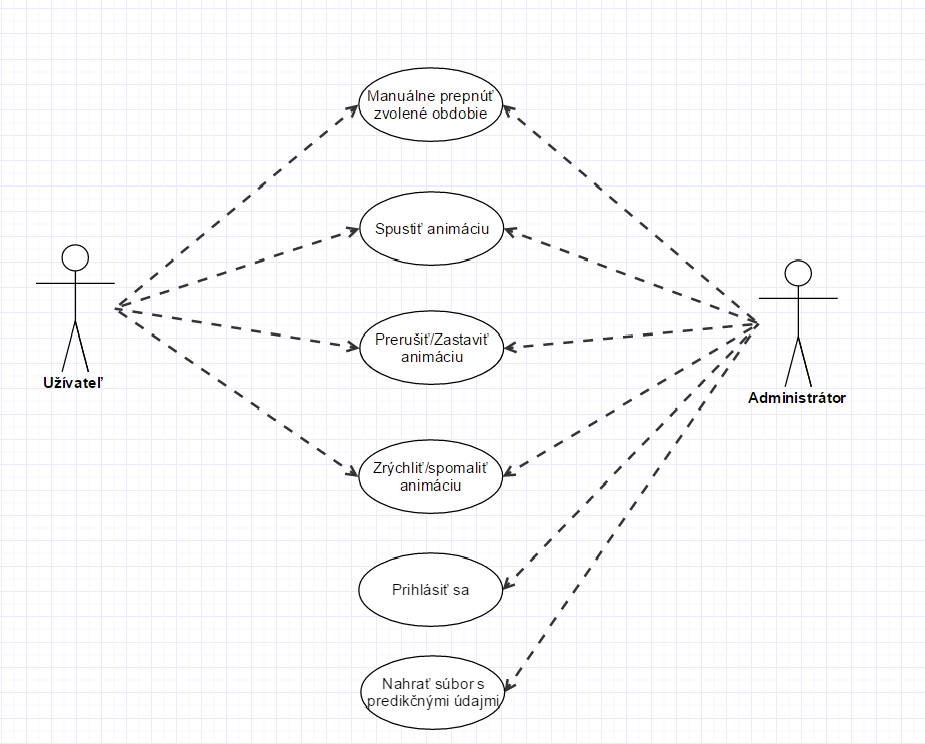
\includegraphics[scale=0.6]{use_case_diagram}
	\caption{Use case diagram}
	\label{fig:Use case diagram}
\end{figure}


\FloatBarrier
\clearpage
\subsection[Entito-relačný diagram]{\rmfamily\bfseries
	Entito-relačný diagram}
Tento diagram je vlastne špeciálnym grafom, ktorý naznačuje vzťahy medzi subjektmi v databáze

\begin{figure}[htb]
	\centering
	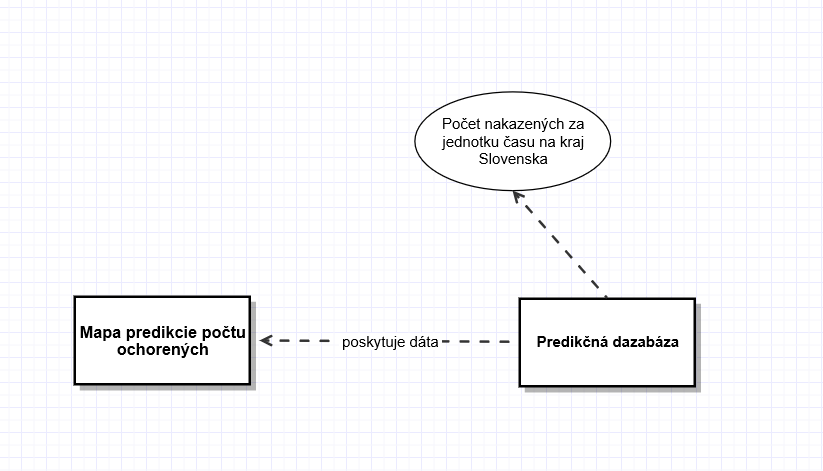
\includegraphics[scale=0.7]{E-R_diagram}
	\caption{Entito-relačný diagram}
	\label{fig:Entito-relačný diagram}
\end{figure}

\FloatBarrier
\end{document}